\documentclass[conference]{IEEEtran}
\IEEEoverridecommandlockouts
\usepackage{cite}
\usepackage[T1]{fontenc}
\usepackage[utf8]{inputenc}
\usepackage{textcomp}

\usepackage{amsmath,amssymb}
\usepackage{graphicx}\graphicspath{{figures/}}
\setkeys{Gin}{keepaspectratio}
\usepackage{booktabs,array,longtable}
\usepackage{adjustbox}
\usepackage{wasysym}
\usepackage{xcolor}
\usepackage{hyperref}
\providecommand{\tightlist}{\setlength{\itemsep}{0pt}\setlength{\parskip}{0pt}}
% placement des flottants : autorise des pages plus riches en figures/tableaux (évite le report en fin d'article)
\renewcommand{\topfraction}{0.9}\renewcommand{\dbltopfraction}{0.9}\renewcommand{\bottomfraction}{0.8}
\renewcommand{\textfraction}{0.07}\renewcommand{\floatpagefraction}{0.85}\renewcommand{\dblfloatpagefraction}{0.85}
\setcounter{topnumber}{3}\setcounter{dbltopnumber}{3}\setcounter{totalnumber}{5}

\usepackage{newunicodechar}
\newunicodechar{●}{\CIRCLE}\newunicodechar{◐}{\LEFTcircle}\newunicodechar{○}{\Circle}
\newunicodechar{≈}{\ensuremath{\approx}}\newunicodechar{≤}{\ensuremath{\leq}}\newunicodechar{≥}{\ensuremath{\geq}}
\newunicodechar{→}{\ensuremath{\rightarrow}}\newunicodechar{−}{\ensuremath{-}}\newunicodechar{θ}{\ensuremath{\theta}}
\newunicodechar{⁻}{\ensuremath{^{-}}}\newunicodechar{⁴}{\ensuremath{^{4}}}\newunicodechar{×}{\ensuremath{\times}}

\begin{document}
\title{Predictive Coordination of Passive and Active Thermal Flexibility in a Multi-Unit Residential Building to Relieve a Distribution Transformer during Winter Peaks}
\author{%
\IEEEauthorblockN{%
Daniel Alain Anyouzo'o $^{1,*}$,
Nilson Henao $^{1}$,
David Toquica $^{1}$,
Alejandro Parrado Duque$^{1}$,\\
Follivi Kloutse $^{3}$,
Olivier Thierry Sosso$^{2}$,
Kodjo Agbossou$^{1}$}
\IEEEauthorblockA{%
$^{1}$Department of Electrical and Computer Engineering, University of Quebec at Trois-Rivieres (UQTR), G8Z 4M3, Canada\\
$^{2}$Hydro-Québec, Montréa, Canada]\\
$^{3}$Department of Electrical Engineering, Advanced Teacher's Training collage for Technical Education, Douala, Cameroon\\
Corresponding author: daniel.alain.anyouzoo@uqtr.ca}%
}

\maketitle
\begin{abstract}
The simultaneous electrification of heating and mobility makes the heat-pump (HP) peak and uncoordinated electric-vehicle (EV) charging coincide on winter evenings at the distribution transformers that supply multi-unit residential buildings. As an alternative to the prohibitive cost of reinforcing distribution-grid infrastructure, this paper proposes a two-layer hierarchical predictive coordination that jointly mobilizes the thermal inertia of the envelope, charged by the HPs (COP ≈ 3) before the peak, and refractory-brick electric thermal storage (ETS) units, which hold a lowered setpoint within the tolerated comfort band during the peak. To create neither an artificial peak nor a rebound, opportunistic ETS recharging is confined under a dynamic power envelope bounded by the off-peak maximum of the reference, and allocated in proportion to the dynamic storage deficit. Each dwelling agent solves a convex optimization problem based on a 4R2C multizone model coupled with a 2R2C ETS model. The physical thermal parameters of the model are calibrated recursively by an extended Kalman filter (EKF), fed with data from a digital twin of the building modeled in BEopt. The distributed hierarchical coordination strategy relies on two layers, namely an aggregator and agents (HEMS). The aggregator coordinates flexibility through a sequential automaton whose phases follow a signal based on a scarcity index that combines the transformer loading and its normalized aging rate (IEEE Std C57.91-2025). The case study addresses the digital twin of a 16-unit building supplied by a 50 kVA transformer over 72 hours. On a −17 °C day, the strategy reduces the peak by 19.3 \%, lowers the maximum hot-spot temperature from 86.4 to 62.4 °C and removes 99 \% of the discomfort, at the cost of a 4.5 \% increase in daily energy.
\end{abstract}
\begin{IEEEkeywords}
Distribution transformer, electric thermal storage, electric vehicles, model predictive control, multi-unit residential buildings, thermal flexibility, valley filling.
\end{IEEEkeywords}

\section*{Nomenclature}
\addcontentsline{toc}{section}{Nomenclature}

\emph{\textbf{{Indices and sets}}}

\par\noindent{\scriptsize\begin{tabular}{@{}>{\raggedright\arraybackslash}p{0.27\linewidth}@{\hspace{4pt}}>{\raggedright\arraybackslash}p{0.70\linewidth}@{}}
\(n\), \(j\in\mathcal A_n\), \(p\), \(k\) & dwelling, adjacent dwelling, floor, time step \\
\(\mathcal C\), \(\sigma\) & congestion set; off-congestion period \\
\end{tabular}}\par\smallskip

\emph{\textbf{Transformer}}

\par\noindent{\scriptsize\begin{tabular}{@{}>{\raggedright\arraybackslash}p{0.27\linewidth}@{\hspace{4pt}}>{\raggedright\arraybackslash}p{0.70\linewidth}@{}}
\(S_n\), PF, \(K_s\) & rated power (kVA); power factor; safety margin \\
\(K\), \(R\) & load factor \(S/S_n\); ratio of load to no-load losses \\
\(P_{lim}\) & active-power limit \((1-K_s)S_n\mathrm{PF}\) (kW) \\
\(\theta_a\), \(\theta_{TO}\), \(\theta_{HS}\) & ambient, top-oil and hot-spot temperatures (°C) \\
\(\Delta\theta_{TO,R}\), \(\Delta\theta_{H,R}\) & rated top-oil and hot-spot rises (K) \\
\(\tau_{TO}\), \(\tau_w\) & oil and winding time constants \\
\(n\), \(m\) & oil and winding exponents (ONAN) \\
\(F_{AA}\), \%LoL & aging acceleration factor; loss of life (\%) \\
\end{tabular}}\par\smallskip

\emph{\textbf{Dwelling and electric thermal storage (ETS})}

\par\noindent{\scriptsize\begin{tabular}{@{}>{\raggedright\arraybackslash}p{0.27\linewidth}@{\hspace{4pt}}>{\raggedright\arraybackslash}p{0.70\linewidth}@{}}
\(T_{i}\), \(T_{e}\), \(T_{ext}\) & indoor-air, envelope and outdoor temperatures (°C) \\
\(T_{h,p}\), \(\alpha\) & corridor temperature of floor \(p\); outdoor weight \\
\(T_{c}\), \(T_{s}\) & ETS brick-core and casing temperatures \\
\(C_i\), \(C_e\), \(C_c\), \(C_s\) & heat capacities: air, envelope, core, ETS casing (J/K) \\
\(R_i\), \(R_o\) & air--envelope and envelope--outdoor resistances (K/W) \\
\(R_{jn}\), \(R_h\) & resistances to the adjacent dwelling and to the corridor \\
\(R_c\), \(R_s\), \(R^{min}_{conv}\) & core--casing, casing--air and minimum forced-convection resistances \\
\(P_h\), COP & HP electric power; coefficient of performance \\
\(P_{ETS}\), \(Q_{ETS}\) & ETS charging power; heat released by the ETS (W) \\
\(Q_{int}\), \(Q_0\) & occupancy gains; identified unmeasured internal gain \\
\(A_s\), \(I_{gh}\) & equivalent solar aperture (m²); global horizontal irradiance (W/m²) \\
SOC, \(T^{min}_c\), \(T^{max}_c\) & ETS state of charge; core temperature bounds \\
\(\beta\), \(\xi\), \(\psi\) & log-parameters; EKF augmented state; noise standard deviations \\
\end{tabular}}\par\smallskip

\emph{\textbf{Coordination and control}}

\par\noindent{\scriptsize\begin{tabular}{@{}>{\raggedright\arraybackslash}p{0.27\linewidth}@{\hspace{4pt}}>{\raggedright\arraybackslash}p{0.70\linewidth}@{}}
\(P_B\), \(P_{nf}\), \(P_{coord}\) & reference load S0; non-flexible load (base + EV); coordinated load S1 \\
\(E\), \(L_\sigma\), \(W_\sigma\) & dynamic envelope; valley-filling level; required recharge energy \\
\(M\), \(c_n\) & building recharge margin; power cap of agent \(n\) \\
\(\gamma_n\), \(\gamma^r_n\), \(G_n\) & fixed share; dynamic recharge share; conductance to unheated zones \\
\(\lambda\), \(\lambda_{pl}\) & scarcity index; floor cost \\
\(T^{ref}\), \(T^{set}\), \(T^{min}\) & reference and effective setpoints; comfort floor \\
\(T_j\), \(\Delta T_n\) & daytime setpoint; night setback \\
\(\Delta_{pre}\), \(\Delta_{eff}\), \(\delta\) & preheating offset; peak setback; comfort tolerance \\
\(\Delta t\), \(H\) & sampling period; prediction horizon (steps) \\
\end{tabular}}\par\smallskip

\section{\textbf{Introduction}}

The simultaneous electrification of heating and transport increases and synchronizes residential demand. In low-voltage networks, the joint deployment of HPs and EV chargers overloads distribution transformers \cite{NavarroEspinosa2016}. Uncoordinated charging concentrates in the early evening \cite{Muratori2018}. Moreover, transformers, which are the bottlenecks of the network, undergo several overload-related stresses, the main consequence of which is aging, governed by the hot-spot temperature through an Arrhenius law \cite{IEEEC5791_2025, IEC60076_7_2018}. Coordinated charging can mitigate this acceleration \cite{Hilshey2013}, and demand response combined with dynamic thermal rating increases the transformer reserve \cite{Daminov2021}. A poorly designed coordination may, however, \textbf{worsen} congestion: price-based scheduling of HPs and EVs synchronizes flexible loads to the point of exceeding the uncoordinated peak \cite{Hein2026}. Relieving the transformer without reinforcement therefore calls on the building itself.

\textbf{The thermal flexibility} of buildings offers two sources:

\begin{itemize}
\tightlist
\item
  \textbf{Passive.} The envelope mass shifts heating \cite{LeDreau2016}; in Québec, an MPC that preheats dwellings reduces the peak by about 30 \% compared with deadband control \cite{Vallianos2023}, and near-optimal setpoint control cuts the peak of electrically heated schools by 40--65 \% \cite{Morovat2022}.
\item
  \textbf{Active.} Refractory-brick ETS units charge a massive core off-peak and release heat through controlled convection \cite{Guzman2015, Devia2021}. Their combination with building mass has been studied for single-family houses \cite{EtedadiAliabadi2022}.
\end{itemize}

Mobilizing these sources at building scale then requires coordinating them. \textbf{Distributed coordination} of HEMS via ADMM enforces a common power limit \cite{Etedadi2023}. Multizone MPC has been applied to dwellings and small buildings \cite{Frahm2025, Hasrat2025}. For deferrable loads, valley filling is the reference for decentralized EV charging \cite{Gan2013}. Table~\ref{tab:I} positions these works against five criteria.

\begin{table*}[tb]
\centering\footnotesize
\caption{Positioning (● addressed; ◐ partially; ○ not addressed; × not addressed, single dwelling; -- not applicable).}\label{tab:I}
\begin{tabular}{>{\raggedright\arraybackslash}p{\dimexpr0.171\linewidth-2\tabcolsep\relax}>{\raggedright\arraybackslash}p{\dimexpr0.143\linewidth-2\tabcolsep\relax}>{\raggedright\arraybackslash}p{\dimexpr0.169\linewidth-2\tabcolsep\relax}>{\raggedright\arraybackslash}p{\dimexpr0.150\linewidth-2\tabcolsep\relax}>{\raggedright\arraybackslash}p{\dimexpr0.182\linewidth-2\tabcolsep\relax}>{\raggedright\arraybackslash}p{\dimexpr0.174\linewidth-2\tabcolsep\relax}}
\toprule
\textbf{Work} & \textbf{Coupled multizone MUB} & \textbf{Passive + active, coordinated} & \textbf{Transformer constraint} & \textbf{No-new-peak guarantee (trajectory)} & \textbf{Coordination} \\
\midrule
\cite{Etedadi2023} & × & ○ (passive only) & fixed limit & ◐ (instantaneous) & iterative ADMM \\
\cite{EtedadiAliabadi2022} & × & ◐ (not coordinated) & ○ & ○ & distributed \\
\cite{Vallianos2023, Morovat2022} & × & ◐ & ○ (price) & ○ & MPC / rules \\
\cite{Frahm2025, Hasrat2025} & ● & ◐ & ○ & ○ & local / central MPC \\
\cite{Daminov2021} & -- & ○ & thermal (DTR) & ◐ & centralized \\
\cite{Gan2013} & -- & -- & ○ & ● (EV) & decentralized \\
\textbf{This work} & \textbf{●} & \textbf{●} & \textbf{fixed limit + aging} & \textbf{● (Prop. 1)} & \textbf{hierarchical, non-iterative} \\
\bottomrule
\end{tabular}
\end{table*}

Table~\ref{tab:I} reveals four gaps. \textbf{G1.} MUBs are usually modeled as a single zone, which neglects heat exchange between adjacent dwellings and with the corridor \cite{Cui2023}. Inter-unit couplings are rarely identified in a verifiable way. \textbf{G2.} Passive (envelope, COP ≈ 3) and active (ETS, COP = 1) flexibility are rarely \emph{ordered} according to their efficiency at multi-dwelling scale. \textbf{G3.} Thermal-storage recharging is left to the local optimizer. Existing architectures guarantee an instantaneous limit, but not the absence of a new peak or rebound over the whole trajectory \cite{Hein2026}. \textbf{G4.} The transformer constraint is rarely linked to its thermal state.

To address these gaps, the contributions of this paper are:

\begin{enumerate}
\def\labelenumi{\arabic{enumi}.}
\tightlist
\item
  a coupled 4R2C multizone dwelling model with a 2R2C ETS model, identified in three steps (augmented-state EKF, output error, maximum likelihood) with an identifiability condition for inter-unit couplings (G1);
\item
  a dynamic setpoint that \textbf{orders} the sources by efficiency (night setback, HP preheating of the envelope, then ETS-held peak setback) with \emph{adaptive} HP curtailment (G2);
\item
  an \textbf{opportunistic recharge envelope} (bounded valley filling, dynamic deficit-based allocation) that provably creates neither an artificial peak nor a rebound (Proposition 1) (G3);
\item
  a 72 h evaluation for a 50 kVA transformer down to −17 °C that reveals the \textbf{physical ceiling} of thermal peak shaving and links coordination to the hot-spot temperature and loss of life (G4, partially).
\end{enumerate}

Section II presents the transformer, dwelling and ETS models and their identification, Section III the coordination, Section IV the case study, Section V the results; Section VI concludes.

\section{\textbf{Modeling}}

The proposed coordination relies on three building blocks: the transformer model, which defines the constraint (II-A); the dwelling and ETS model, which describes the available flexibility (II-B); and the identification procedure that sets its parameters (II-C).

\subsection{Transformer Thermal Model}

We use the method of §7.3.8, Eq. (48), of IEEE Std C57.91-2025 \cite{IEEEC5791_2025}, consistent with IEC 60076-7 \cite{IEC60076_7_2018}. With \(K=S/S_n\) the load factor, and for \(K\) constant over a step \(\Delta t\), the discrete solution reads:

\begin{equation}\label{eq:1}
\adjustbox{max width=\linewidth}{$\displaystyle \begin{aligned}\theta_{TO}(k{+}1)&=\theta^{ss}_{TO}(k)+\big(\theta_{TO}(k)-\theta^{ss}_{TO}(k)\big)e^{-\Delta t/\tau_{TO}},\\ \theta^{ss}_{TO}&=\theta_a+\Delta\theta_{TO,R}\Big[\tfrac{K^2R+1}{R+1}\Big]^n\end{aligned}$}
\end{equation}

\begin{equation}\label{eq:2}
\adjustbox{max width=\linewidth}{$\displaystyle \begin{aligned}\Delta\theta_{H}(k{+}1)&=\Delta\theta_{H,R}K^{2m}+\big(\Delta\theta_{H}(k)-\Delta\theta_{H,R}K^{2m}\big)e^{-\Delta t/\tau_{w}},\\ \theta_{HS}&=\theta_{TO}+\Delta\theta_H\end{aligned}$}
\end{equation}

with \(n=m=0.8\) for ONAN cooling (Table 6 of the standard). This exact form is unconditionally stable and removes the criterion \(\Delta t\le\tau_w/2\) (§7.3.9) of explicit schemes. For thermally upgraded paper \cite{IEEEC5791_2025}:

\begin{equation}\label{eq:3}
\adjustbox{max width=\linewidth}{$\displaystyle \begin{aligned}F_{AA}&=\exp\!\Big(\frac{15\,000}{383.15}-\frac{15\,000}{\theta_{HS}+273.15}\Big),\\ \%LoL&=\frac{100}{180\,000}\sum_kF_{AA}(k)\Delta t\end{aligned}$}
\end{equation}

The normal-life limits are \(\theta_{HS}\le120\) °C and \(\theta_{TO}\le105\) °C. This model provides the grid-side constraint; the building-side flexibility is described next.

\subsection{Multizone Dwelling and ETS Model}

Each dwelling \(n\) is described by its indoor air (\(T_{i,n}\)) and envelope (\(T_{e,n}\)). It is coupled to the adjacent dwelling \(j\in\mathcal A_n\), to the corridor \(T_{h,p}\) and to its ETS (core \(T_{c,n}\), insulated casing \(T_{s,n}\)), as shown in Fig.~\ref{fig:1} \cite{Bacher2011, Belic2021}:

\begin{equation}\label{eq:4}
\adjustbox{max width=\linewidth}{$\displaystyle C_{e,n}\dot T_{e,n}=\frac{T_{ext}-T_{e,n}}{R_{o,n}}+\frac{T_{i,n}-T_{e,n}}{R_{i,n}}$}
\end{equation}

\begin{equation}\label{eq:5}
\adjustbox{max width=\linewidth}{$\displaystyle \begin{aligned}C_{i,n}\dot T_{i,n}={}&\frac{T_{e,n}-T_{i,n}}{R_{i,n}}+\sum_{j\in\mathcal A_n}\frac{T_{i,j}-T_{i,n}}{R_{jn}}+\frac{T_{h,p}-T_{i,n}}{R_{h,n}}\\&+\frac{T_{s,n}-T_{i,n}}{R_{s,n}}+\mathrm{COP}\,P_{h,n}+Q_{ETS,n}+Q_{int,n}\end{aligned}$}
\end{equation}

\begin{equation}\label{eq:6}
\adjustbox{max width=\linewidth}{$\displaystyle \begin{aligned}C_{c,n}\dot T_{c,n}&=P_{ETS,n}-Q_{ETS,n}-\frac{T_{c,n}-T_{s,n}}{R_{c,n}},\\ C_{s,n}\dot T_{s,n}&=\frac{T_{c,n}-T_{s,n}}{R_{c,n}}-\frac{T_{s,n}-T_{i,n}}{R_{s,n}}\end{aligned}$}
\end{equation}

\begin{equation}\label{eq:7}
\adjustbox{max width=\linewidth}{$\displaystyle \begin{aligned}&0\le Q_{ETS,n}\le\min\Big\{Q^{max}_{ETS},\frac{T_{c,n}-T_{i,n}}{R^{min}_{conv}}\Big\},\\ &\mathrm{SOC}_n=\frac{T_{c,n}-T^{min}_c}{T^{max}_c-T^{min}_c}\end{aligned}$}
\end{equation}

where \(T_{h,p}=\alpha T_{ext}+\frac{1-\alpha}{|\mathcal N_p|}\sum_{j\in\mathcal N_p}T_{i,j}\) for the corridor of floor \(p\) and \(C_{c,n}=m_c c_p\) (brick mass and specific heat). The storage discharge \(Q_{ETS,n}\) is a control input bounded by constraint \eqref{eq:7}, evaluated at the current state, which preserves convexity \cite{Guzman2015, Devia2021}. With state \(x_n=[T_{c},T_{s},T_{i},T_{e}]^\top\), input \(u_n=[P_{h},Q_{ETS},P_{ETS}]^\top\) and disturbances \(d_n=[T_{ext},Q_{int},T_{h,p},T_{i,j}]^\top\), the linear system \eqref{eq:4}--\eqref{eq:6} is discretized exactly with a zero-order hold (exponential of the augmented matrix):

\begin{equation}\label{eq:8}
\adjustbox{max width=\linewidth}{$\displaystyle \begin{aligned}&x_n(k{+}1)=A_dx_n(k)+B_du_n(k)+E_dd_n(k),\\ &\begin{bmatrix}A_d&[B_d\ E_d]\\0&I\end{bmatrix}=\exp\!\Big(\begin{bmatrix}A&[B\ E]\\0&0\end{bmatrix}\Delta t\Big)\end{aligned}$}
\end{equation}

\begin{figure}[tb]
\centering
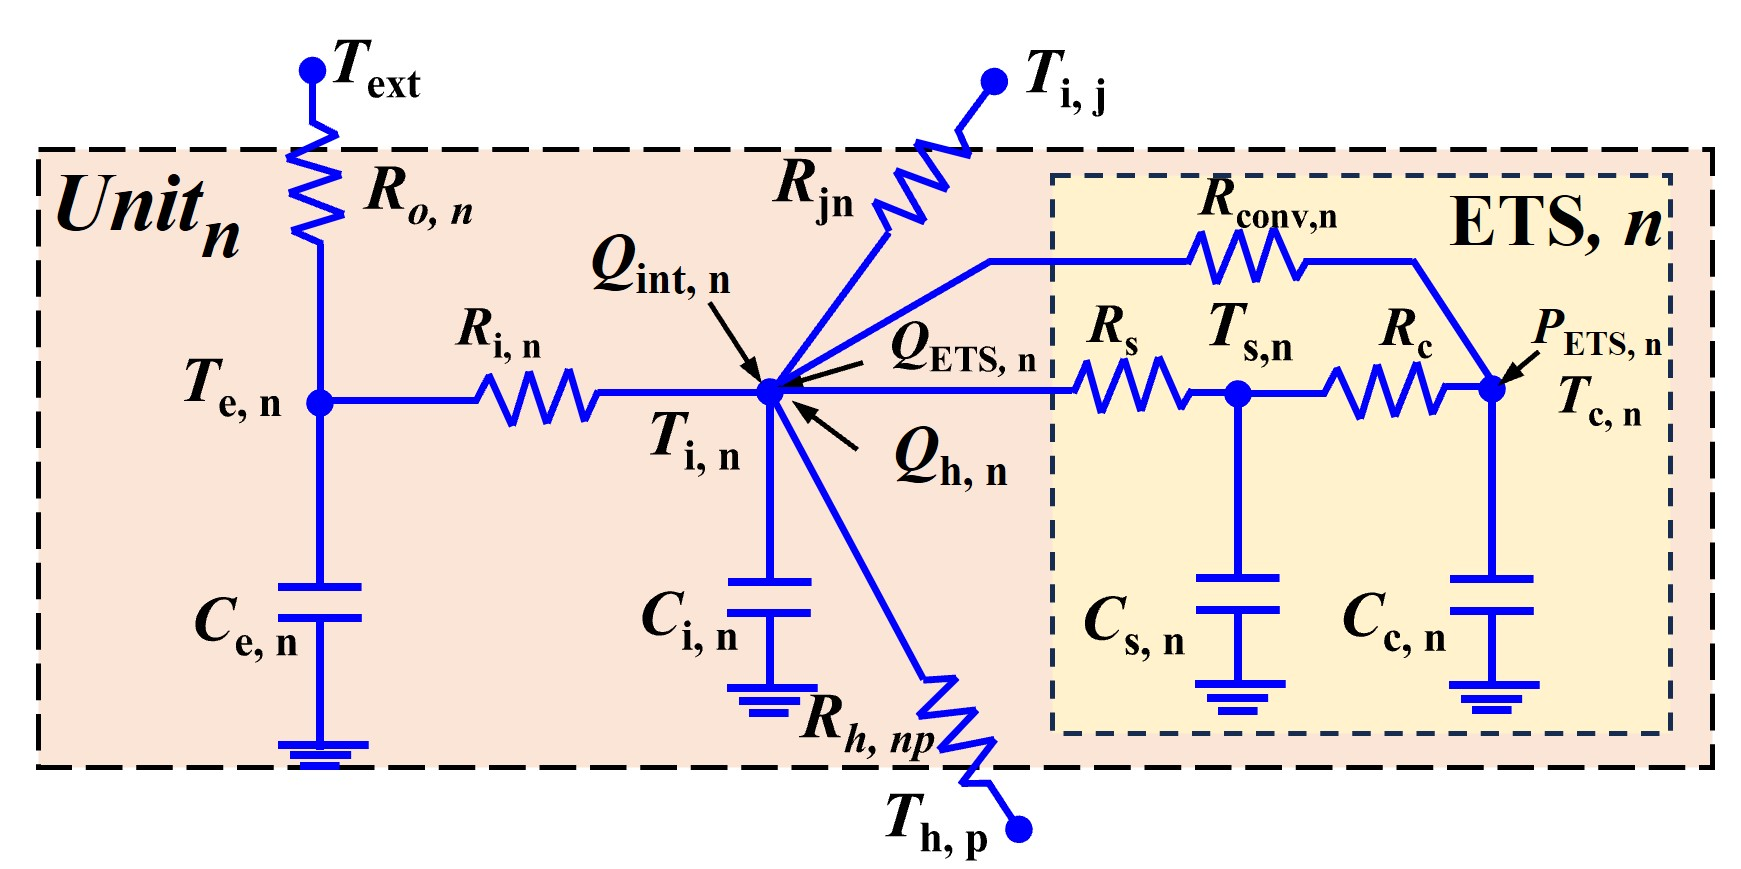
\includegraphics[width=0.82\linewidth,]{fig1_rc.jpg}
\caption{Coupled RC model of a dwelling (4R2C) and its ETS (2R2C + controlled discharge). Dwelling nodes: air \(T_{i,n}\) and envelope \(T_{e,n}\); ETS nodes: core \(T_{core}\equiv T_c\) and casing \(T_{env}\equiv T_s\); controlled discharge through \(R_{conv}\). Branches \(R_{jn}\) and \(R_{h,np}\) connect the dwelling to its neighbor and to the corridor.}
\label{fig:1}
\end{figure}

The capacitances and resistances of \eqref{eq:4}--\eqref{eq:5} cannot be measured directly and must be identified.

\subsection{Identification of the Thermal Parameters}

\textbf{Data.} The data come from a BEopt 2.8.0 digital twin (Standard mode, new construction, multi-family) \cite{BEopt28} built on EnergyPlus, with the 2011--2025 TMYx weather file of Trois-Rivières \cite{OneBuilding2025}. The typical floor and its RC reduction are shown in Fig.~\ref{fig:2}. For each dwelling, two one-month experiments are simulated (January, hourly): \(\mathcal E_1\), variable PRBS setpoint heating (pulsed reheats to 25 °C followed by free decays), and \(\mathcal E_2\), free-floating.

\begin{figure}[tb]
\centering
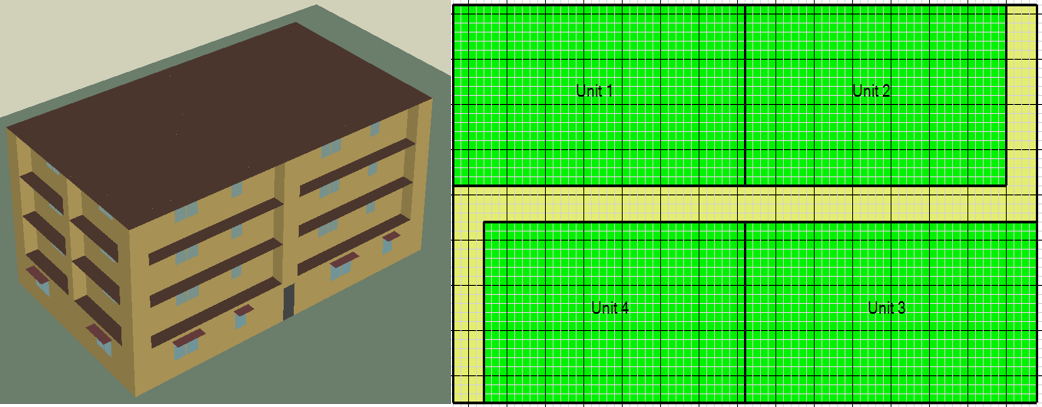
\includegraphics[width=0.85\linewidth,]{fig2_beopt.png}
\caption{3D view of the BEopt digital twin model of the 16-unit MUB building distributed over four floors}
\label{fig:2}
\end{figure}

\begin{figure}[tb]
\centering
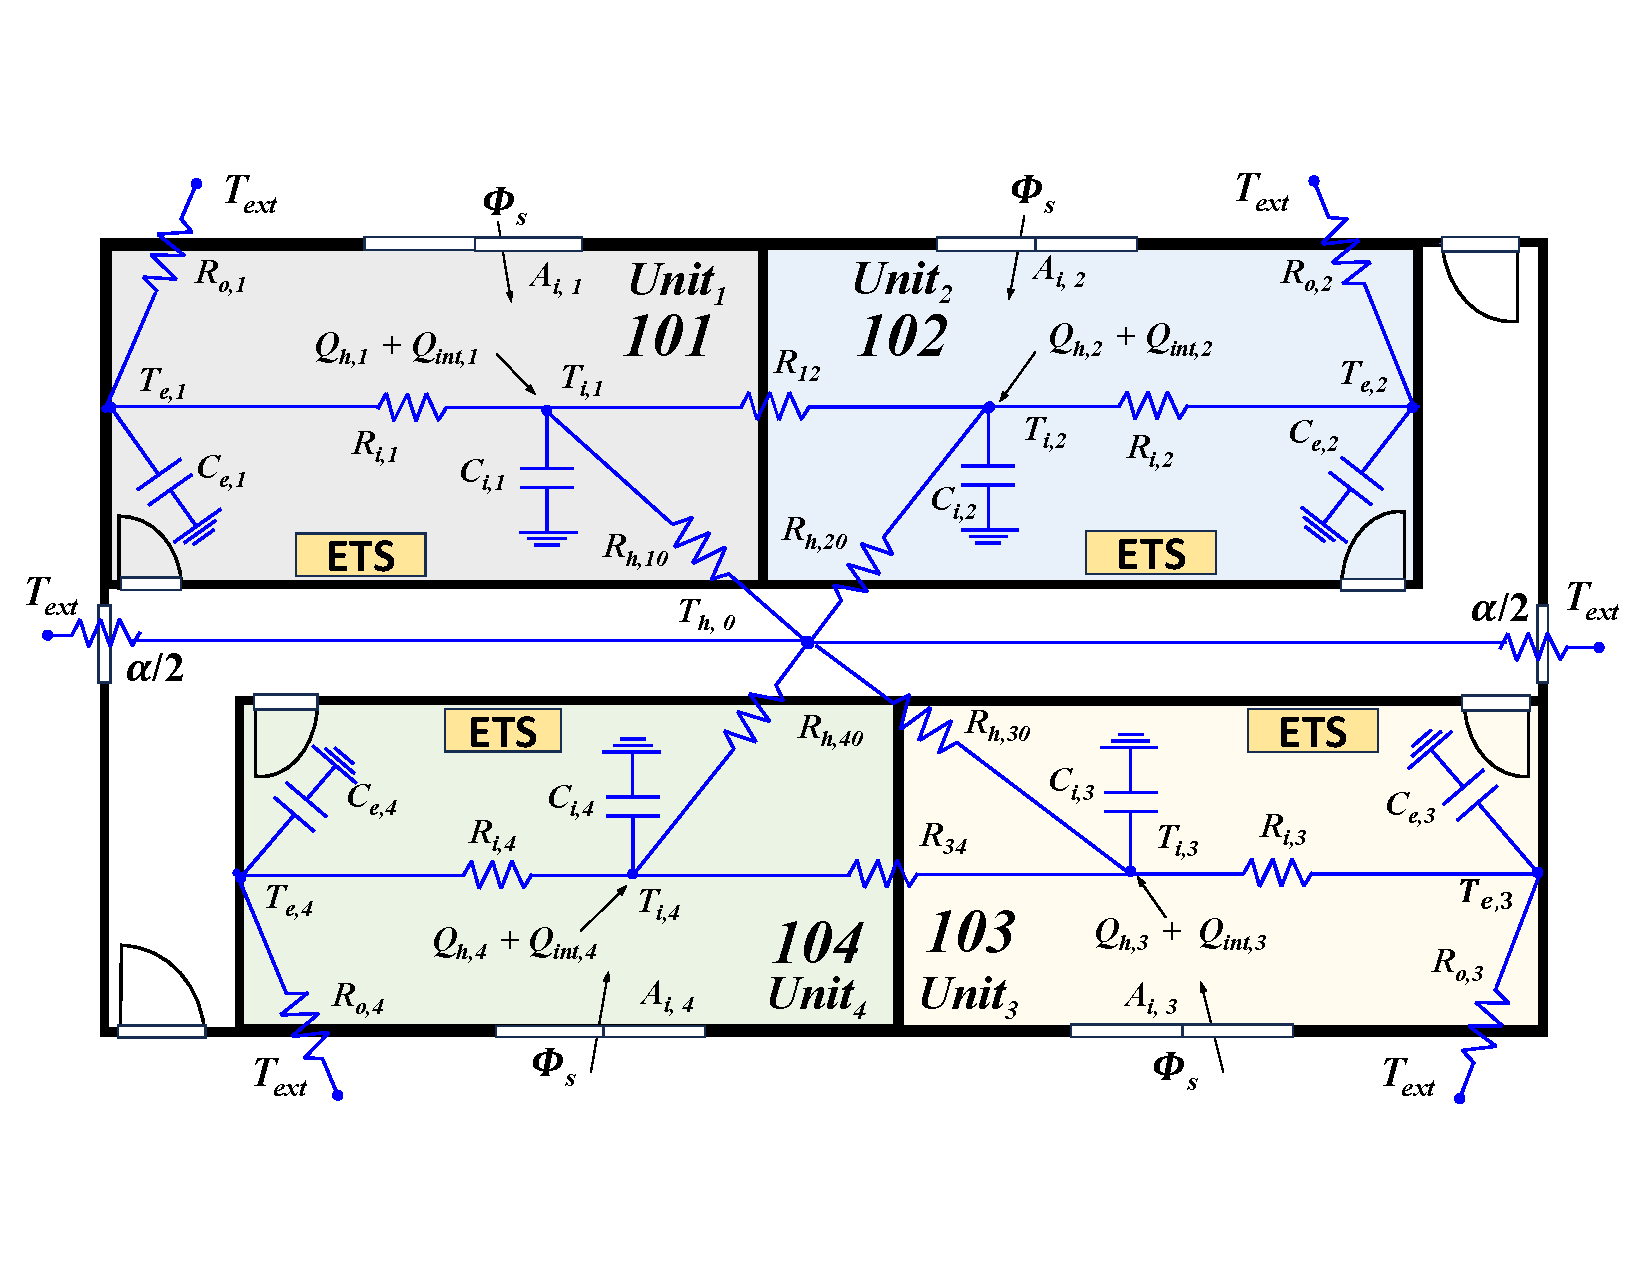
\includegraphics[width=0.95\linewidth,]{fig3_palier.pdf}
\caption{2D view and reduced 4R2C model of a unit of floor \(p\) of the MUB (units 101--104, central corridor): party-wall couplings \(R_{12}\), \(R_{34}\), corridor couplings \(R_{h,n0}\) and solar apertures \(A_{i,n}\).}
\label{fig:3}
\end{figure}

\begin{figure}[tb]
\centering
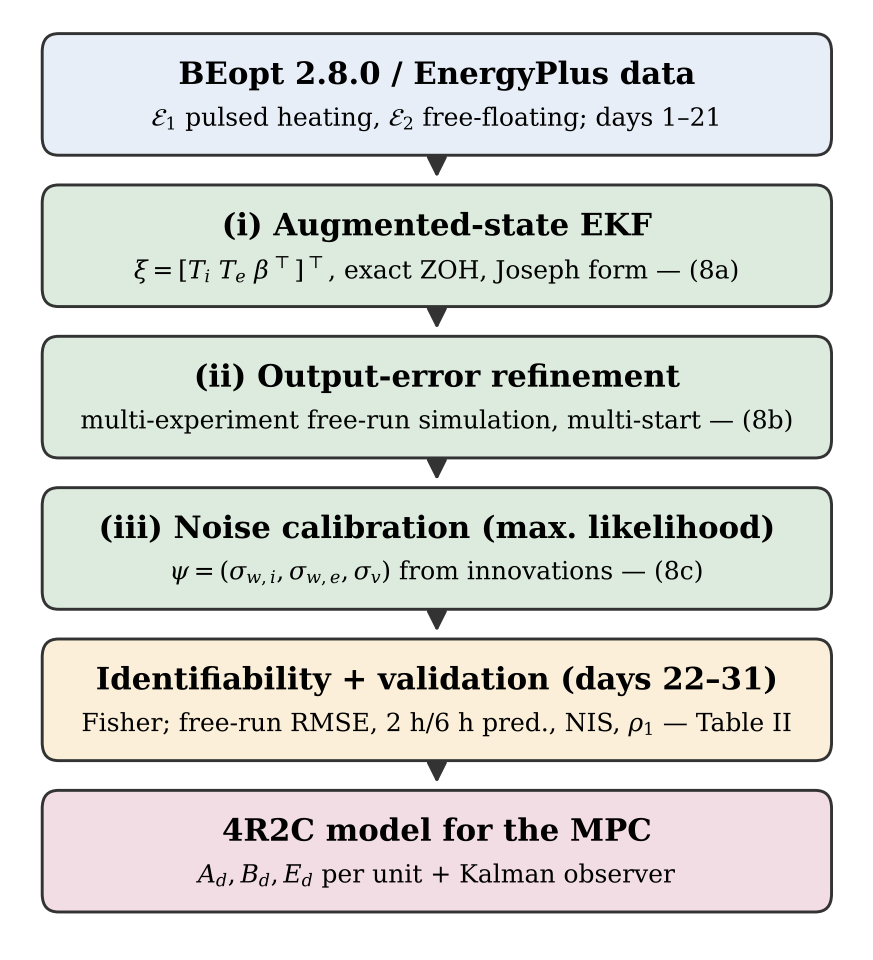
\includegraphics[width=0.88\linewidth,]{fig4_ident.png}
\caption{Identification framework: augmented-state Extended Kalman Filter (EKF), output-error refinement, noise covariance tuning through maximum likelihood estimation, followed by an identifiability analysis and out-of-sample validation.}
\label{fig:4}
\end{figure}

\textbf{Identification model.} Identification is decoupled: neighbor and corridor temperatures are measured inputs \cite{Belic2021}. Sub-model \eqref{eq:4}--\eqref{eq:5}, without ETS, is augmented with two input coefficients: an equivalent solar aperture \(A_s\) applied to the global horizontal irradiance \(I_{gh}\), and an unmeasured internal gain \(Q_0\). These coefficients do not modify the dynamics \(A_d\) used by the controller. The free parameters \(\beta=\log[R_i\ R_o\ C_i\ C_e\ A_s\ Q_0]\) are estimated in log scale, which guarantees positivity and balances magnitudes; the model is discretized exactly by \eqref{eq:8}.

\textbf{Three-step estimation.} (i) An augmented-state EKF on \(\xi_k=[T_i\ T_e\ \beta^\top]^\top\), where \(\beta\) follows a slow random walk, jointly estimates states and parameters from \(T_i\) only, the two experiments being chained \cite{Fux2014, Kristensen2004}; (ii) its overconfident estimate initializes an \textbf{output-error} (free-run) least-squares refinement, the relevant criterion for a prediction model \cite{Harb2016}; (iii) the observer noise covariances are calibrated by maximum likelihood of the innovations \cite{Kristensen2004}.

\textbf{Identifiability and protocol.} The Fisher information matrix \cite{Raue2009} yields two results. First, BEopt applies the same setpoint to all units (mean neighbor difference 0.48 °C); since the sensitivity of \(T_i\) to \(R_{jn}\) is driven by \(T_{i,j}-T_{i,n}\), \(R_{jn}\) and \(R_h\) are not excited and are fixed at their geometric values. Second, on \(\mathcal E_1\) alone, losses and gains are confounded (\(r(R_o,Q_0)=-0.97\)); multi-experiment calibration on days 1--21 of \(\mathcal E_1\) and \(\mathcal E_2\) brings \(|r|\) down to 0.74--0.90 \cite{Bacher2011}. Validation on days 22--31 covers free-run simulation, 2 h (MPC horizon) and 6 h prediction with the Kalman observer, and observer consistency (NIS, lag-1 innovation autocorrelation \(\rho_1\)) (Table~\ref{tab:II}).

\begin{table*}[tb]
\centering\footnotesize
\caption{Identification on the test window (days 22--31); predictions, NIS and \(\rho_1\): averages over \(\mathcal E_1\) and \(\mathcal E_2\).}\label{tab:II}
\begin{tabular}{>{\raggedright\arraybackslash}p{\dimexpr0.165\linewidth-2\tabcolsep\relax}>{\raggedright\arraybackslash}p{\dimexpr0.196\linewidth-2\tabcolsep\relax}>{\raggedright\arraybackslash}p{\dimexpr0.196\linewidth-2\tabcolsep\relax}>{\raggedright\arraybackslash}p{\dimexpr0.132\linewidth-2\tabcolsep\relax}>{\raggedright\arraybackslash}p{\dimexpr0.132\linewidth-2\tabcolsep\relax}>{\raggedright\arraybackslash}p{\dimexpr0.070\linewidth-2\tabcolsep\relax}>{\raggedright\arraybackslash}p{\dimexpr0.100\linewidth-2\tabcolsep\relax}}
\toprule
\textbf{Dwellings} & \textbf{RMSE \(\mathcal E_1\) (°C); \(R^2\)} & \textbf{RMSE \(\mathcal E_2\) (°C); \(R^2\)} & \textbf{2 h pred. (°C)} & \textbf{6 h pred. (°C)} & \textbf{NIS} & \textbf{\(\rho_1\)} \\
\midrule
Ground floor (101--104) & 1.56; 0.74 & 1.66; 0.70 & 0.78 & 1.00 & 0.87 & 0.10 \\
Upper floors (201--404) & 1.07; 0.90 & 0.96; 0.94 & 0.78 & 0.95 & 0.95 & 0.13 \\
\bottomrule
\end{tabular}
\end{table*}

On upper floors, all criteria are met. On the ground floor, the uninsulated slab couples the dwelling to the ground, which the 4R2C model does not represent: the free-run error is higher, but the prediction error at the MPC horizon remains below 0.8 °C because the observer corrects the state at every step. The validated model is the one used by each local agent of the coordination described next.

\section{\textbf{Hierarchical Coordination}}

The hierarchical coordination architecture is organized in two layers (Fig.~\ref{fig:3}): the first is the \textbf{grid aggregator}, located at the distribution transformer; the second consists of the \textbf{local HEMS-MPC agents}, installed in each apartment and described by Fig.~\ref{fig:1}. The aggregator computes \emph{ex ante} the index \(\lambda\), the automaton phases and the envelope \(E(k)\), then allocates the margins; each HEMS-MPC agent optimizes its dwelling; a guard filter checks the aggregate. Subsections A--E follow the order of these computations.

\begin{figure}[tb]
\centering
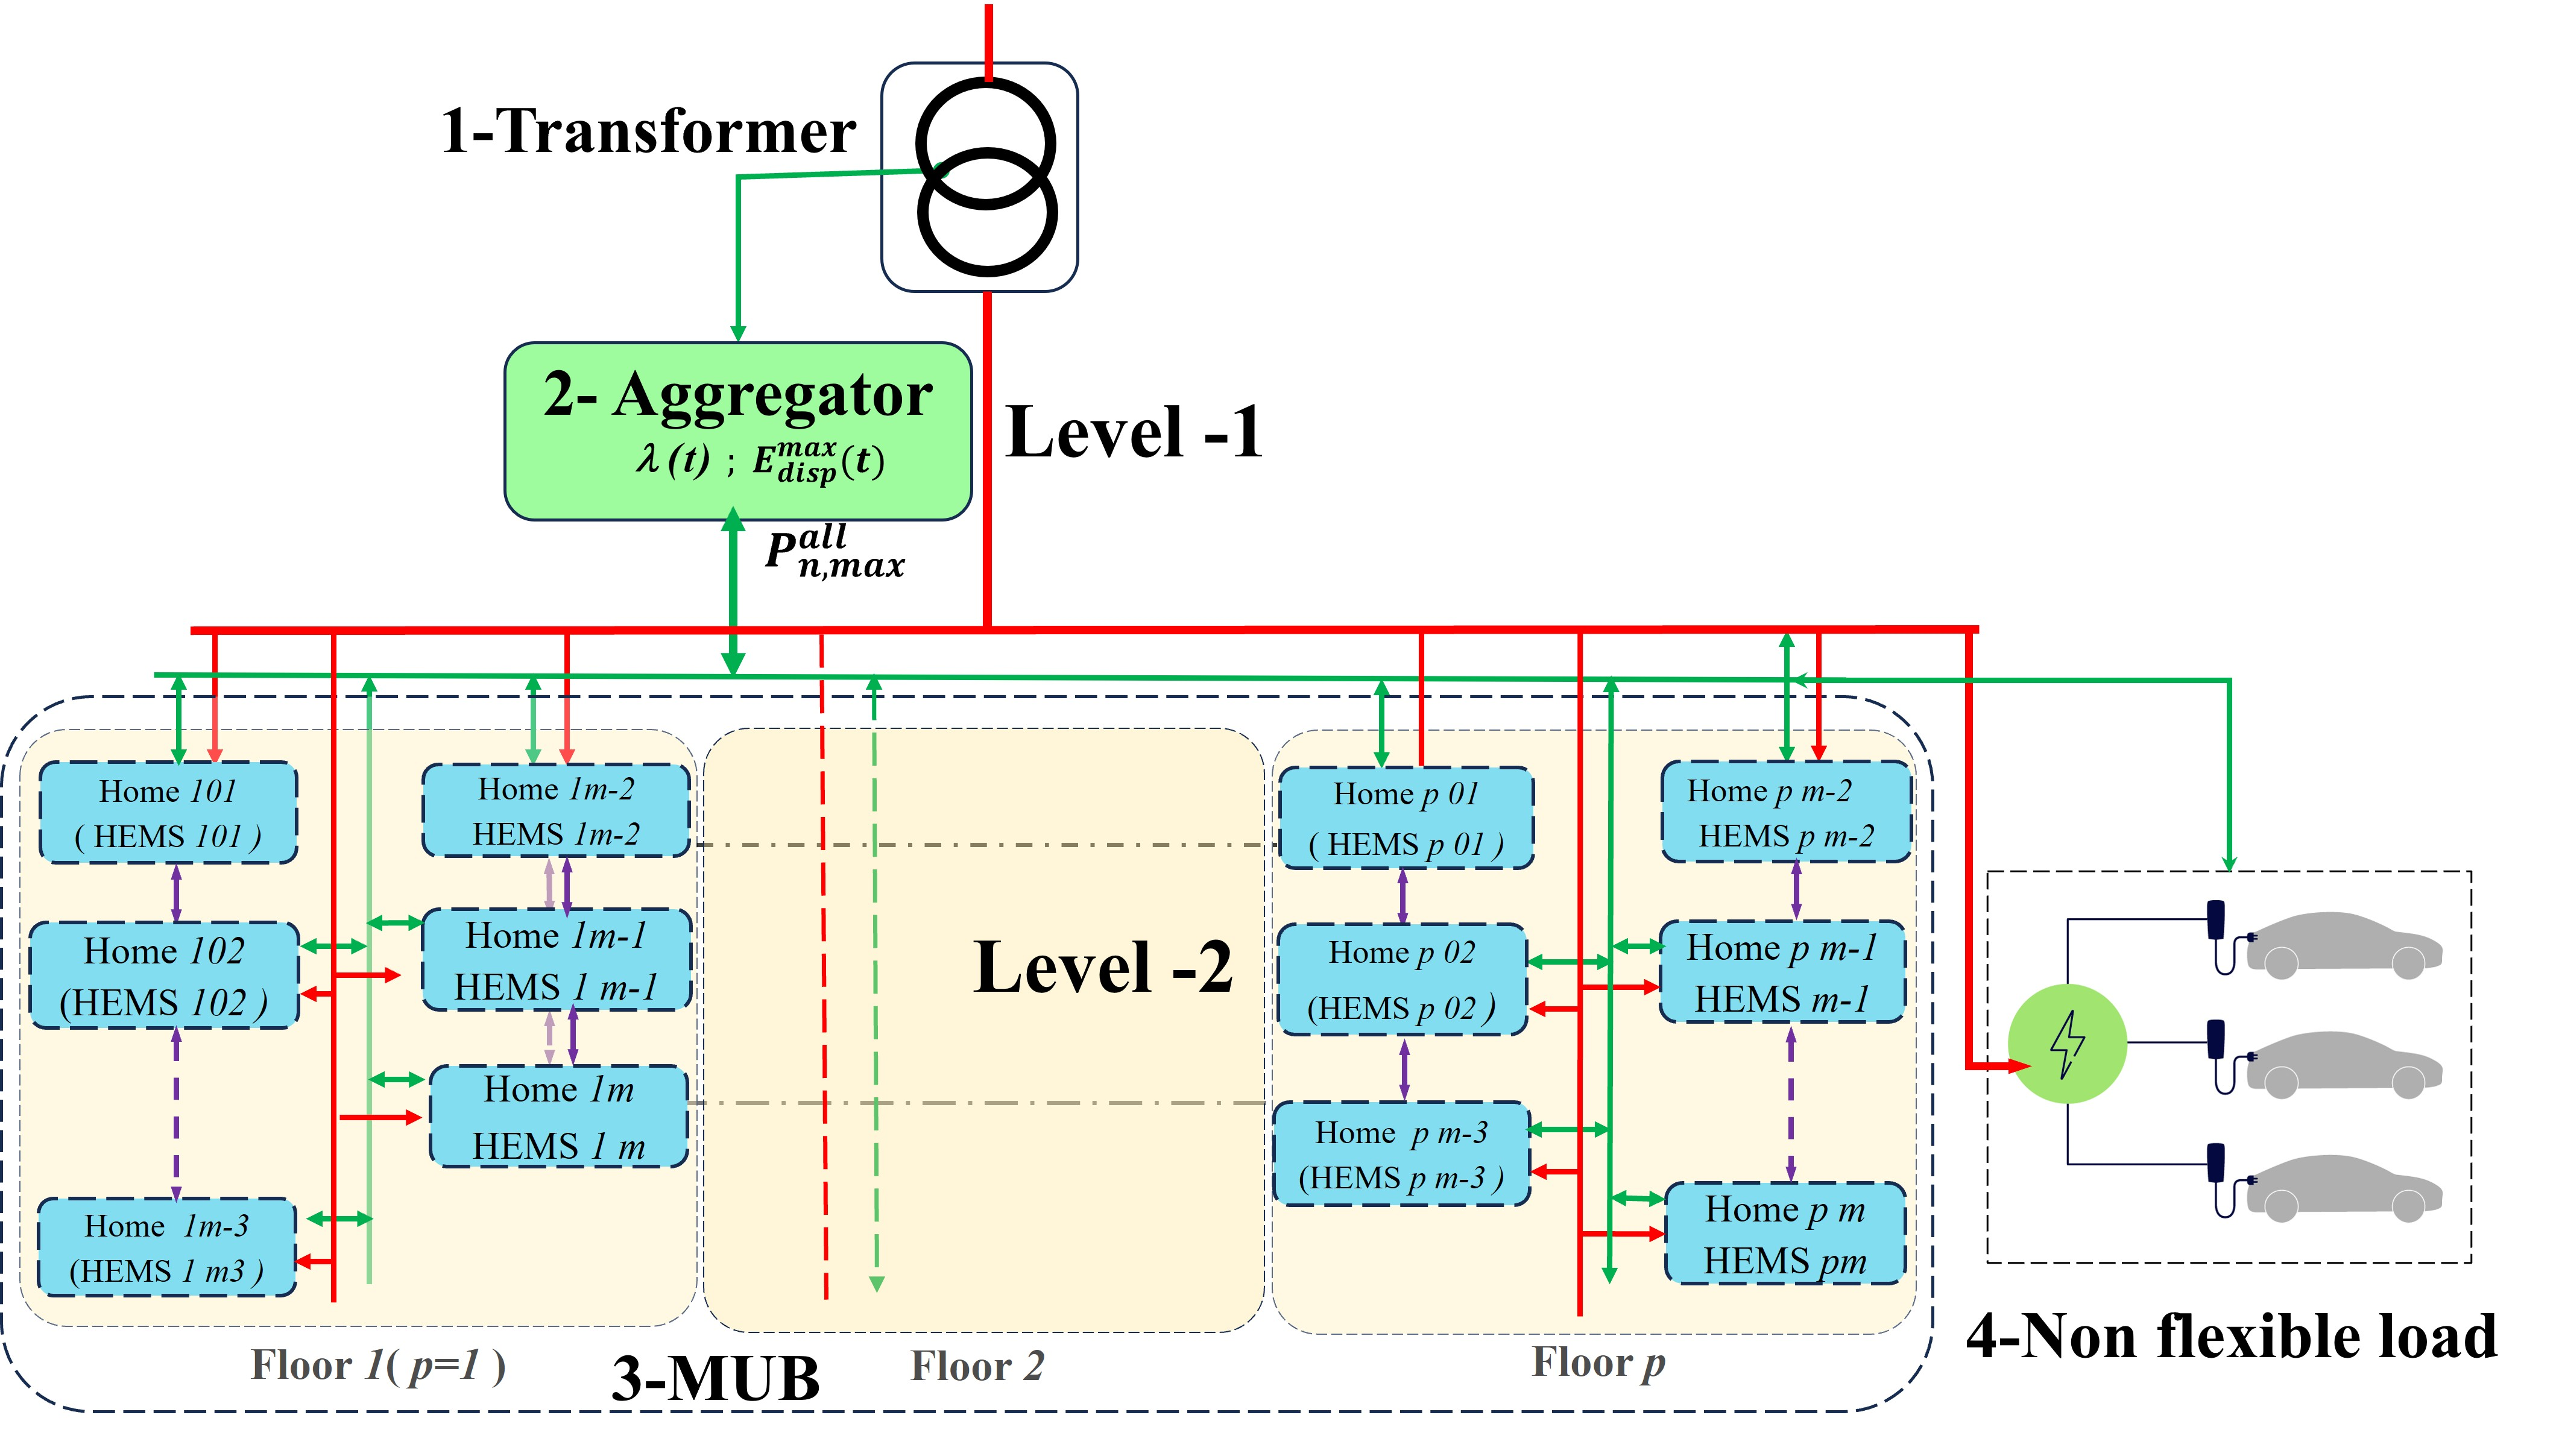
\includegraphics[width=0.88\linewidth,]{fig4_arch.jpg}
\caption{Coordination architecture: two layers; the aggregator, at the transformer, broadcasts the index \(\lambda(t)\) and the power cap \(c_n\equiv P^{max}_{disp}(t)\) to the HEMS agents of each dwelling and floor; EV charging remains uncoordinated.}
\label{fig:5}
\end{figure}

\subsection{Reference Trajectory and Scarcity Index}

The aggregator first simulates the uncoordinated reference trajectory \(P_B(k)=P_{nf}(k)+\sum_nP^B_{h,n}(k)\), where \(P_{nf}\) gathers the aggregated base load of the MUB and EV charging, and \(P^B_{h,n}\) is the power of PID-controlled HPs tracking the same reference setpoint (Section III-B). This trajectory, assumed perfectly forecast, feeds \eqref{eq:1}--\eqref{eq:2} and the dimensionless index:

\begin{equation}\label{eq:9}
\adjustbox{max width=\linewidth}{$\displaystyle \begin{aligned}\lambda(k)={}&w_L\min\Big\{1,e^{\kappa(u(k)-1)}\Big\}+w_T\min\Big\{1,\frac{F_{AA}(\theta^B_{HS}(k))}{F_{AA}(120\,^\circ\mathrm{C})}\Big\},\\ &u=P_B/P_{lim},\quad P_{lim}=(1-K_s)S_n\mathrm{PF}\end{aligned}$}
\end{equation}

with \(w_L+w_T=1\), which guarantees \(\lambda\in[0,1]\). The first term equals 1 at the safety limit and decays exponentially below it; the second is the \textbf{normalized aging rate}, equal to 1 when the predicted hot spot reaches 120 °C. It is broadcast over the horizon with a floor cost \(\lambda_{pl}\), so that off-peak energy is not free and HP efficiency is valued against the ETS. The index tells \emph{when} the grid is constrained; the dynamic setpoint defines \emph{how} dwellings respond.

\subsection{Dynamic Setpoint: Night Setback, Preheating and Peak Setback}

The reference setpoint applies the night setback recommended in Canada---a 2--3 °C reduction during sleep \cite{RNCan2024}:

\begin{equation}\label{eq:10}
\adjustbox{max width=\linewidth}{$\displaystyle T^{ref}(k)=\begin{cases}T_j & h(k)\in[\,6{:}00,\,22{:}01)\\ T_j-\Delta T_n,\ \Delta T_n\le3\text{ °C} & \text{otherwise}\end{cases}$}
\end{equation}

The automaton (Section III-C) then modulates the effective setpoint sent to the agents:

\begin{equation}\label{eq:11}
\adjustbox{max width=\linewidth}{$\displaystyle \begin{aligned}&T^{set}(k)=\begin{cases}T^{ref}+\Delta_{pre} & \text{preheating}\\ \min\{T^{ref},\,T_j-\Delta_{eff}\} & \text{congestion}\\ T^{ref} & \text{otherwise}\end{cases}\\ &T^{min}(k)=T^{set}(k)-\delta\end{aligned}$}
\end{equation}

This sequence orders the sources by efficiency. Before the peak, the HP (COP ≈ 3) stores heat in the envelope mass by raising the setpoint by \(\Delta_{pre}\). During the peak, the setpoint is lowered by \(\Delta_{eff}\) within the tolerated band: the free decay of \(T_i\) releases the heat stored in the envelope, then the ETS (COP = 1) holds the lowered setpoint. The \(\min\{\cdot\}\) prevents the peak setback from adding to the night setback when congestion extends beyond 22:01. Switching between setpoints is decided by the phase automaton.

\subsection{Phase Automaton and Adaptive Curtailment}

Phases are determined \emph{ex ante} on the reference. The congestion set is \(\mathcal C=\{k:P_B(k)\ge P_{lim}\}\), from which exceedances shorter than \(\tau_{min}\) are removed (e.g., the morning reheat after the night setback); these are handled by the envelope (Section III-D) with \(E(k)=\max\{P_{lim},P_{nf}(k)\}\). Table~\ref{tab:III} summarizes the bounds imposed at each horizon step \(j\), so that each agent knows the upcoming curtailment periods in advance.

\begin{table*}[tb]
\centering\footnotesize
\caption{Phase automaton (evaluated at each horizon step).}\label{tab:III}
\begin{tabular}{>{\raggedright\arraybackslash}p{\dimexpr0.144\linewidth-2\tabcolsep\relax}>{\raggedright\arraybackslash}p{\dimexpr0.269\linewidth-2\tabcolsep\relax}>{\raggedright\arraybackslash}p{\dimexpr0.242\linewidth-2\tabcolsep\relax}>{\raggedright\arraybackslash}p{\dimexpr0.335\linewidth-2\tabcolsep\relax}}
\toprule
\textbf{Phase} & \textbf{Condition} & \textbf{Setpoint} & \textbf{Bounds imposed on agent \(n\)} \\
\midrule
0 Normal & none of the others & \(T^{ref}\) & \(P_h+P_{ETS}\le c_n\) (16); \(P_{ETS}\le\gamma^r_nM\); \(Q_{ETS}=0\) \\
1 Preheating & congestion within the next \(J_{pre}\) steps & \(T^{ref}+\Delta_{pre}\) & same as phase 0 \\
2 Congestion & \(k\in\mathcal C\) & \(\min\{T^{ref},T_j-\Delta_{eff}\}\) & \(P_h\le\gamma_n[P_{lim}-P_{nf}]^+\); \(P_{ETS}=0\); \(Q_{ETS}\) by (7) \\
3 Recovery & \(J_{rep}\) steps after congestion & \(T^{ref}\) & \(P_h\le\gamma_n[E-P_{nf}]^+\); \(P_{ETS}=0\); \(Q_{ETS}\) by (7) \\
\bottomrule
\end{tabular}
\end{table*}

During congestion, the HP is not switched off but limited to its share of the residual transformer margin, allocated in proportion to each dwelling's conductance to unheated zones:

\begin{equation}\label{eq:12}
\adjustbox{max width=\linewidth}{$\displaystyle \gamma_n=\frac{G_n}{\sum_lG_l},\qquad G_n=\frac{1}{R_{i,n}+R_{o,n}}+\frac{1}{R_{h,n}}$}
\end{equation}

When \(P_{nf}>P_{lim}\), the margin is zero and the coordinated load equals \(P_{nf}\): the peak reduction is then \textbf{bounded by the heating share of the reference peak}, \(\Delta P_{max}/P_{B,max}\le P^B_h(k^*)/P_B(k^*)\). Curtailment, however, creates a storage deficit in the ETS units, which must be refilled off-peak without creating a new peak: this is the role of the recharge envelope.

\subsection{Opportunistic Recharge Envelope}

ETS recharging must create neither an artificial peak nor a rebound, and should exploit the hours when the transformer is lightly loaded. The aggregator defines a dynamic envelope for the coordinated load:

\begin{equation}\label{eq:13}
\adjustbox{max width=\linewidth}{$\displaystyle E(k)=\begin{cases}P_B(k) & k\in\mathcal C\\ \max\big\{P_B(k),\ \min\{sP_{lim},L_\sigma\}\big\} & k\in\sigma\end{cases}$}
\end{equation}

where \(\sigma\) is an off-congestion period (between two congestions) and \(L_\sigma\) its valley-filling level \cite{Gan2013}: the smallest level that makes the required recharge energy \(W_\sigma\) available, bounded by the reference maximum over the period,

\begin{equation}\label{eq:14}
\adjustbox{max width=\linewidth}{$\displaystyle \begin{aligned}L_\sigma&=\min\Big\{L\le\min\big(sP_{lim},\max_{k\in\sigma}P_B(k)\big):\sum_{k\in\sigma}[L-P_B(k)]^+\Delta t\ge W_\sigma\Big\},\\ W_\sigma&=\min\Big\{f_b\,\mathrm{COP}\sum_{k\in\mathcal C_{\sigma}^{+}}\sum_nP^B_{h,n}(k)\Delta t,\ W^{max}\Big\}\end{aligned}$}
\end{equation}

\(\mathcal C^+_\sigma\) is the next congestion, whose heat supplied by the reference HPs must be released by the ETS units; \(f_b>1\) covers standby losses; \(W^{max}\) is the total usable ETS capacity. \(L_\sigma\) is found by bisection, since \(\sum_k[L-P_B]^+\) is monotone in \(L\). At each step, the building recharge margin over the horizon is

\begin{equation}\label{eq:15}
\adjustbox{max width=\linewidth}{$\displaystyle M(k{+}j)=\Big[E(k{+}j)-P_{nf}(k{+}j)-\sum_n\hat P_{h,n}(k{+}j)\Big]^+$}
\end{equation}

where \(\hat P_{h,n}\) is the HP plan of agent \(n\) at the previous step, shifted by one step; heating thus has priority. The total margin is split into a heating part, at the fixed share \(\gamma_n\), and a recharge part, at the \textbf{dynamic} share of the storage deficit:

\begin{equation}\label{eq:16}
\adjustbox{max width=\linewidth}{$\displaystyle \begin{aligned}c_n(k{+}j)&=\gamma_n\big[E-P_{nf}-M\big]^++\gamma^r_n(k)\,M,\\ \gamma^r_n(k)&=\frac{\gamma_n[\mathrm{SOC}^\star-\mathrm{SOC}_n(k)]^+}{\sum_l\gamma_l[\mathrm{SOC}^\star-\mathrm{SOC}_l(k)]^+}\end{aligned}$}
\end{equation}

\textbf{Proposition 1 (no artificial peak).} If each agent satisfies \(P_{h,n}+P_{ETS,n}\le c_n\) off congestion and the bounds of Table~\ref{tab:III} during congestion, then for all \(k\): \(P_{coord}(k)\le E(k)\le\max\{P_B(k),\min(sP_{lim},\max_{\sigma}P_B)\}\). Hence the coordinated load never exceeds the reference during congestion and never exceeds, off congestion, the off-peak maximum of the reference.

\emph Off congestion, \(\sum_n\gamma_n=\sum_n\gamma^r_n=1\) and \eqref{eq:16} give \(\sum_nc_n=[E-P_{nf}-M]^++M=E-P_{nf}\) whenever \(E\ge P_{nf}\), hence \(P_{coord}=P_{nf}+\sum_n(P_{h,n}+P_{ETS,n})\le E\). During congestion, \(\sum_nP_{h,n}\le[P_{lim}-P_{nf}]^+\) and \(P_{ETS,n}=0\), hence \(P_{coord}\le\max\{P_{lim},P_{nf}\}\le P_B\). The bound on \(E\) follows from \eqref{eq:13}--\eqref{eq:14}.

A guard filter in the aggregator restores \(P_{coord}(k)\le E(k)\), first by scaling down recharging, if an agent fails to converge.

\textbf{Remark (strict variant).} Imposing \(P_{coord}\le P_B\) at every step (\(L_\sigma=0\)) leaves almost no off-peak margin, since both trajectories track the same setpoint, whereas the heat released by the ETS must be bought back off-peak at COP = 1 (Section V-C). The automaton bounds and the cap \(c_n\) are the only information each local agent receives.

\subsection{Local Model Predictive Control}

With the condensed prediction matrices derived from \eqref{eq:8}, \(T_{i,n}=c_T+G_TU_n\) and \(T_{c,n}(k{+}H)=c_C+g_C^\top U_n\), where \(U_n\in\mathbb R^{3H}\) is the input sequence, each agent solves:

\begin{equation}\label{eq:17}
\adjustbox{max width=\linewidth}{$\displaystyle \begin{aligned}\min_{U_n\ge0}\ &\sum_{j=0}^{H-1}\Big[\tilde\lambda_j(P_{h,n}+P_{ETS,n})\Delta t+\mu_c\,e_j^2+\mu_b\big[T^{min}_j-T_{i,n}\big]_+^2\\&\qquad+\mu_h\big[T_{i,n}-T^{max}_j\big]_+^2+\mu_\Delta\|\Delta u_j\|^2\Big]\\&+\mu_T\big[\mathrm{SOC}^{ref}-\mathrm{SOC}_n(k{+}H)\big]_+^2\end{aligned}$}
\end{equation}

subject to \(u_j\le\bar u_j\) (Table~\ref{tab:III}), \(P_{h,n}+P_{ETS,n}\le c_n(k{+}j)\) and \eqref{eq:7}, with \(e_j=T_{i,n}-T^{set}_j\) and \(\tilde\lambda=\lambda+\lambda_{pl}\). Comfort is relaxed \textbf{asymmetrically} (\(\mu_h\ll\mu_b\)), since being warmer than the lowered setpoint is not discomfort. The terminal term gives stored energy a value (otherwise \(P_{ETS}=0\) is optimal): \(\mathrm{SOC}^{ref}=0\) when the horizon ends in congestion or recovery, \(\mathrm{SOC}^\star\) otherwise, the envelope \eqref{eq:13}--\eqref{eq:16} deciding \emph{when} to recharge. The penalties \([\cdot]_+^2\) are convex and continuously differentiable: \eqref{eq:17} is a convex problem with 36 variables, solved by SQP (SLSQP in SciPy \cite{Virtanen2020}) with an analytic gradient and an explicit envelope constraint. Only \(\tilde\lambda\), \(c_n\), the bounds and \(T^{set}\) are transmitted; no individual data are sent upstream, except the SOC used in \eqref{eq:16}. The next section applies this complete chain to a 16-unit building.

\begin{figure*}[tb]
\centering
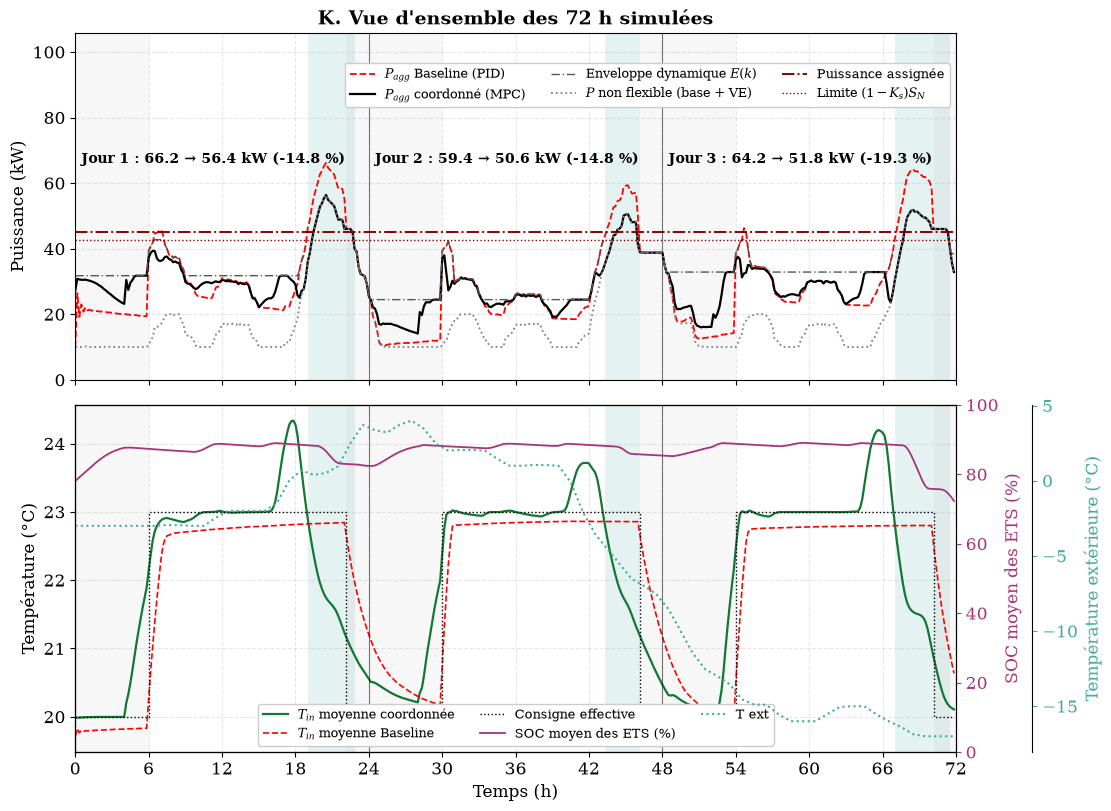
\includegraphics[width=\textwidth]{fig5_72.png}
\caption{Overview of the 72 simulated hours. Top: transformer load for S0 (PID, red dashed) and S1 (coordinated MPC, black), dynamic envelope \(E(k)\), non-flexible load (base + EV, dotted), rated power and limit \((1-K_s)S_n\); green bands: congestion; gray bands: night setback. Bottom: mean indoor temperature for S0 and S1, effective setpoint, mean ETS SOC and outdoor temperature.}
\label{fig:6}
\end{figure*}



\section{\textbf{Case Study}}

The MUB has 16 dwellings on four levels (72 m² on the ground floor, 56 m² on upper floors). The coordination simulations use a \textbf{preliminary RC parameter set} with higher inertia than the set of Table~\ref{tab:II}: envelope time constant \((R_i+R_o)C_e\approx170\) h, versus 72 h on upper floors for the identified set; robustness to the identified set is discussed in Section V-E. The daytime setpoint is \(T_j=23\) °C with a night setback \(\Delta T_n=3\) °C (20 °C from 22:01 to 05:59) \cite{RNCan2024}. Internal gains follow a stochastic occupancy profile \cite{Richardson2008} (100 W per present occupant). The corridor of each floor is modeled algebraically with \(\alpha=0.8\).

The single-phase ONAN 50 kVA transformer (PF = 0.9, i.e., 45 kW) has losses \(P_0=170\) W and \(P_k=390\) W, i.e., \(R=2.29\) (CSA C802). The limit is \(P_{lim}=0.95\times45=42.75\) kW and the ambient temperature \(\theta_a\) is the outdoor temperature. Base-load, EV-charging (up to 36 kW in the early evening) and outdoor-temperature profiles cover 72 h, from mild to cold: day 1 from -3.0 to 3.7 °C, day 2 from -7.9 to 4.0 °C, and day 3, a cold snap, from -17.0 to -8.0 °C. The step is \(\Delta t=600\) s and the horizon \(H=12\) steps (2 h). The three days are analyzed separately; the ETS units start at \(T_c=500\) °C (SOC ≈ 78 \%).

Two scenarios are compared on the same reference setpoint \eqref{eq:10}. \textbf{S0}: PID thermostats (\(K_p=1.9\), \(K_i=0.005\), \(K_d=0.02\), anti-windup), ETS inactive, uncoordinated EVs. \textbf{S1}: the proposed coordination. The strict variant of S1 (\(L_\sigma=0\)) is also evaluated. Table~\ref{tab:IV} lists the parameters.

\begin{table*}[tb]
\centering\footnotesize
\caption{Main parameters.}\label{tab:IV}
\begin{tabular}{>{\raggedright\arraybackslash}p{\dimexpr0.237\linewidth-2\tabcolsep\relax}>{\raggedright\arraybackslash}p{\dimexpr0.753\linewidth-2\tabcolsep\relax}}
\toprule
\textbf{Item} & \textbf{Values} \\
\midrule
HP & \(P^{max}_h=1.8\) kW; COP = 3.0 \\
ETS & \(C_c=105\times1155\) J/K; \(C_s=18\) kJ/K; \(R_c=12\) K/W; \(R_s=6\) K/W; \(T_c\in[150,600]\) °C; \(P^{max}_{ETS}=Q^{max}_{ETS}=2.5\) kW; \(\mathrm{SOC}^\star=0.9\) \\
Transformer & \(S_n=50\) kVA; PF = 0.9; \(K_s=5\) \%; \(\Delta\theta_{TO,R}=55\) K; \(\Delta\theta_{H,R}=25\) K; \(\tau_{TO}=180\) min; \(\tau_w=5\) min; \(n=m=0.8\) \\
Setpoint & \(T_j=23\) °C; \(\Delta T_n=3\) °C; \(\Delta_{pre}=\Delta_{eff}=1.5\) °C; \(\delta=0.5\) °C; \(J_{pre}=2\) h; \(J_{rep}=1\) h; \(\tau_{min}=1\) h \\
Envelope & \(s=0.90\); \(f_b=1.3\) \\
Index \(\lambda\) & \(w_L=0.75\); \(\kappa=8\); \(\lambda_{pl}=0.30\); \(w_T=0.25\) \\
MPC & \(\mu_c=2\); \(\mu_b=500\); \(\mu_h=2\); \(\mu_\Delta=0.05\); \(\mu_T=200\) \\
\bottomrule
\end{tabular}
\end{table*}

\textbf{Indicators.} The peak window is set on S0. Rebound is the S1 energy above S0 during recovery and the following 2 h; valley-filling energy is the remaining off-peak excess. The daily energy of S1 is corrected for the change in ETS storage over the day, valued at COP = 1. Discomfort is the integral, summed over dwellings, of \([T^{min}-T_{i,n}]^+\). The flexibility contribution index (FCI) of a dwelling is its share of the \(\lambda\)-weighted net curtailment; fairness is measured by Jain's index \cite{Jain1984} of the ratio FCI\(/\gamma_n\).

\section{\textbf{Results and Discussion}}

\begin{table}[tb]
\centering\footnotesize
\caption{Summary of indicators per day (S0 → S1).}\label{tab:V}
\begin{tabular}{>{\raggedright\arraybackslash}p{\dimexpr0.328\linewidth-2\tabcolsep\relax}>{\raggedright\arraybackslash}p{\dimexpr0.221\linewidth-2\tabcolsep\relax}>{\raggedright\arraybackslash}p{\dimexpr0.221\linewidth-2\tabcolsep\relax}>{\raggedright\arraybackslash}p{\dimexpr0.221\linewidth-2\tabcolsep\relax}}
\toprule
\textbf{Indicator} & \textbf{Day 1} & \textbf{Day 2} & \textbf{Day 3} \\
\midrule
Peak \(\max P\) (kW) & 66.2 → 56.4 & 59.4 → 50.6 & 64.2 → 51.8 \\
Reduction; heating share (\%) & 14.8; 14.8 & 14.8; 14.8 & 19.3; 19.3 \\
Curtailed energy; rebound (kWh) & 37.6; 0.0 & 24.7; 0.0 & 45.6; 0.0 \\
\(\max(P_{coord}-E)\) (kW) & 0.00 & 0.00 & 0.00 \\
Off-peak maximum (kW) & 41.8 → 39.9 & 42.6 → 38.9 & 41.8 → 40.3 \\
\(\max\theta_{HS}\) (°C) & 101.5 → 83.3 & 87.9 → 71.5 & 86.4 → 62.4 \\
Discomfort (°C·h) & 14.94 → 2.74 & 10.83 → 0.34 & 12.22 → 0.11 \\
ETS recharge (kWh\(_e\)); off-peak share (\%) & 37.3; 74 & 23.8; 83 & 16.7; 88 \\
ETS discharge (kWh\(_{th}\)); min SOC (\%) & 11.9; 66 & 4.6; 66 & 37.1; 54 \\
Corrected energy (kWh); change (\%) & 769.2 → 782.2; +1.7 & 644.4 → 653.5; +1.4 & 753.0 → 786.6; +4.5 \\
Jain's index & 0.980 & 0.991 & 0.997 \\
\bottomrule
\end{tabular}
\end{table}

\subsection{Peak Reduction and Physical Ceiling}

Every evening, the reference peak occurs at 20:30, when EV charging (up to 36 kW) adds to the base load and the HPs (Fig.~\ref{fig:4}). Coordination reduces it from 66.2 to 56.4 kW (−14.8 \%) on day 1, from 59.4 to 50.6 kW (−14.8 \%) on day 2 and from 64.2 to 51.8 kW (−19.3 \%) on day 3 (Table~\ref{tab:V}). In all three cases, the reduction is \textbf{exactly equal} to the heating share of the reference peak, and the coordinated peak coincides with the maximum of \(P_{nf}\). At peak time, the non-flexible load alone exceeds \(P_{lim}\): the margin in \eqref{eq:12} is zero, the HPs are fully curtailed and thermal flexibility is exhausted. The coordinated peak therefore remains above \(P_{lim}\) (load factor 1.15 on day 3) and the overload duration only drops from 4.7 to 3.7 h. This \textbf{physical ceiling} is structural: beyond it, only acting on EV charging or a dynamic thermal constraint can reduce the peak further.

\subsection{Envelope-then-ETS Sequence}

Fig.~\ref{fig:5} details day 3. Preheating by 1.5 °C precedes congestion (Fig.~\ref{fig:4}, bottom, around 17:00--19:00); during congestion, the free decay of \(T_i\) toward the lowered setpoint first releases the envelope heat, then the ETS takes over (Fig.~\ref{fig:5}-C, discharge in magenta). The electric energy curtailed during the peak reaches 45.6 kWh, i.e., about 137 kWh of heat at COP 3; the ETS discharge supplies 37.1 kWh\(_{th}\) of it, the rest coming from the envelope and the setpoint reduction. The corrected energy increase (+1.4 to +4.5 \%) reflects the HP → ETS substitution (COP 3 → 1), moderated by the envelope support at COP 3. Comfort is \textbf{improved} (−82 to −99 \% discomfort), mainly because the MPC anticipates the 06:00 reheat that the PID performs as a delayed step (Fig.~\ref{fig:4}, bottom).

\begin{figure*}[tb]
\centering
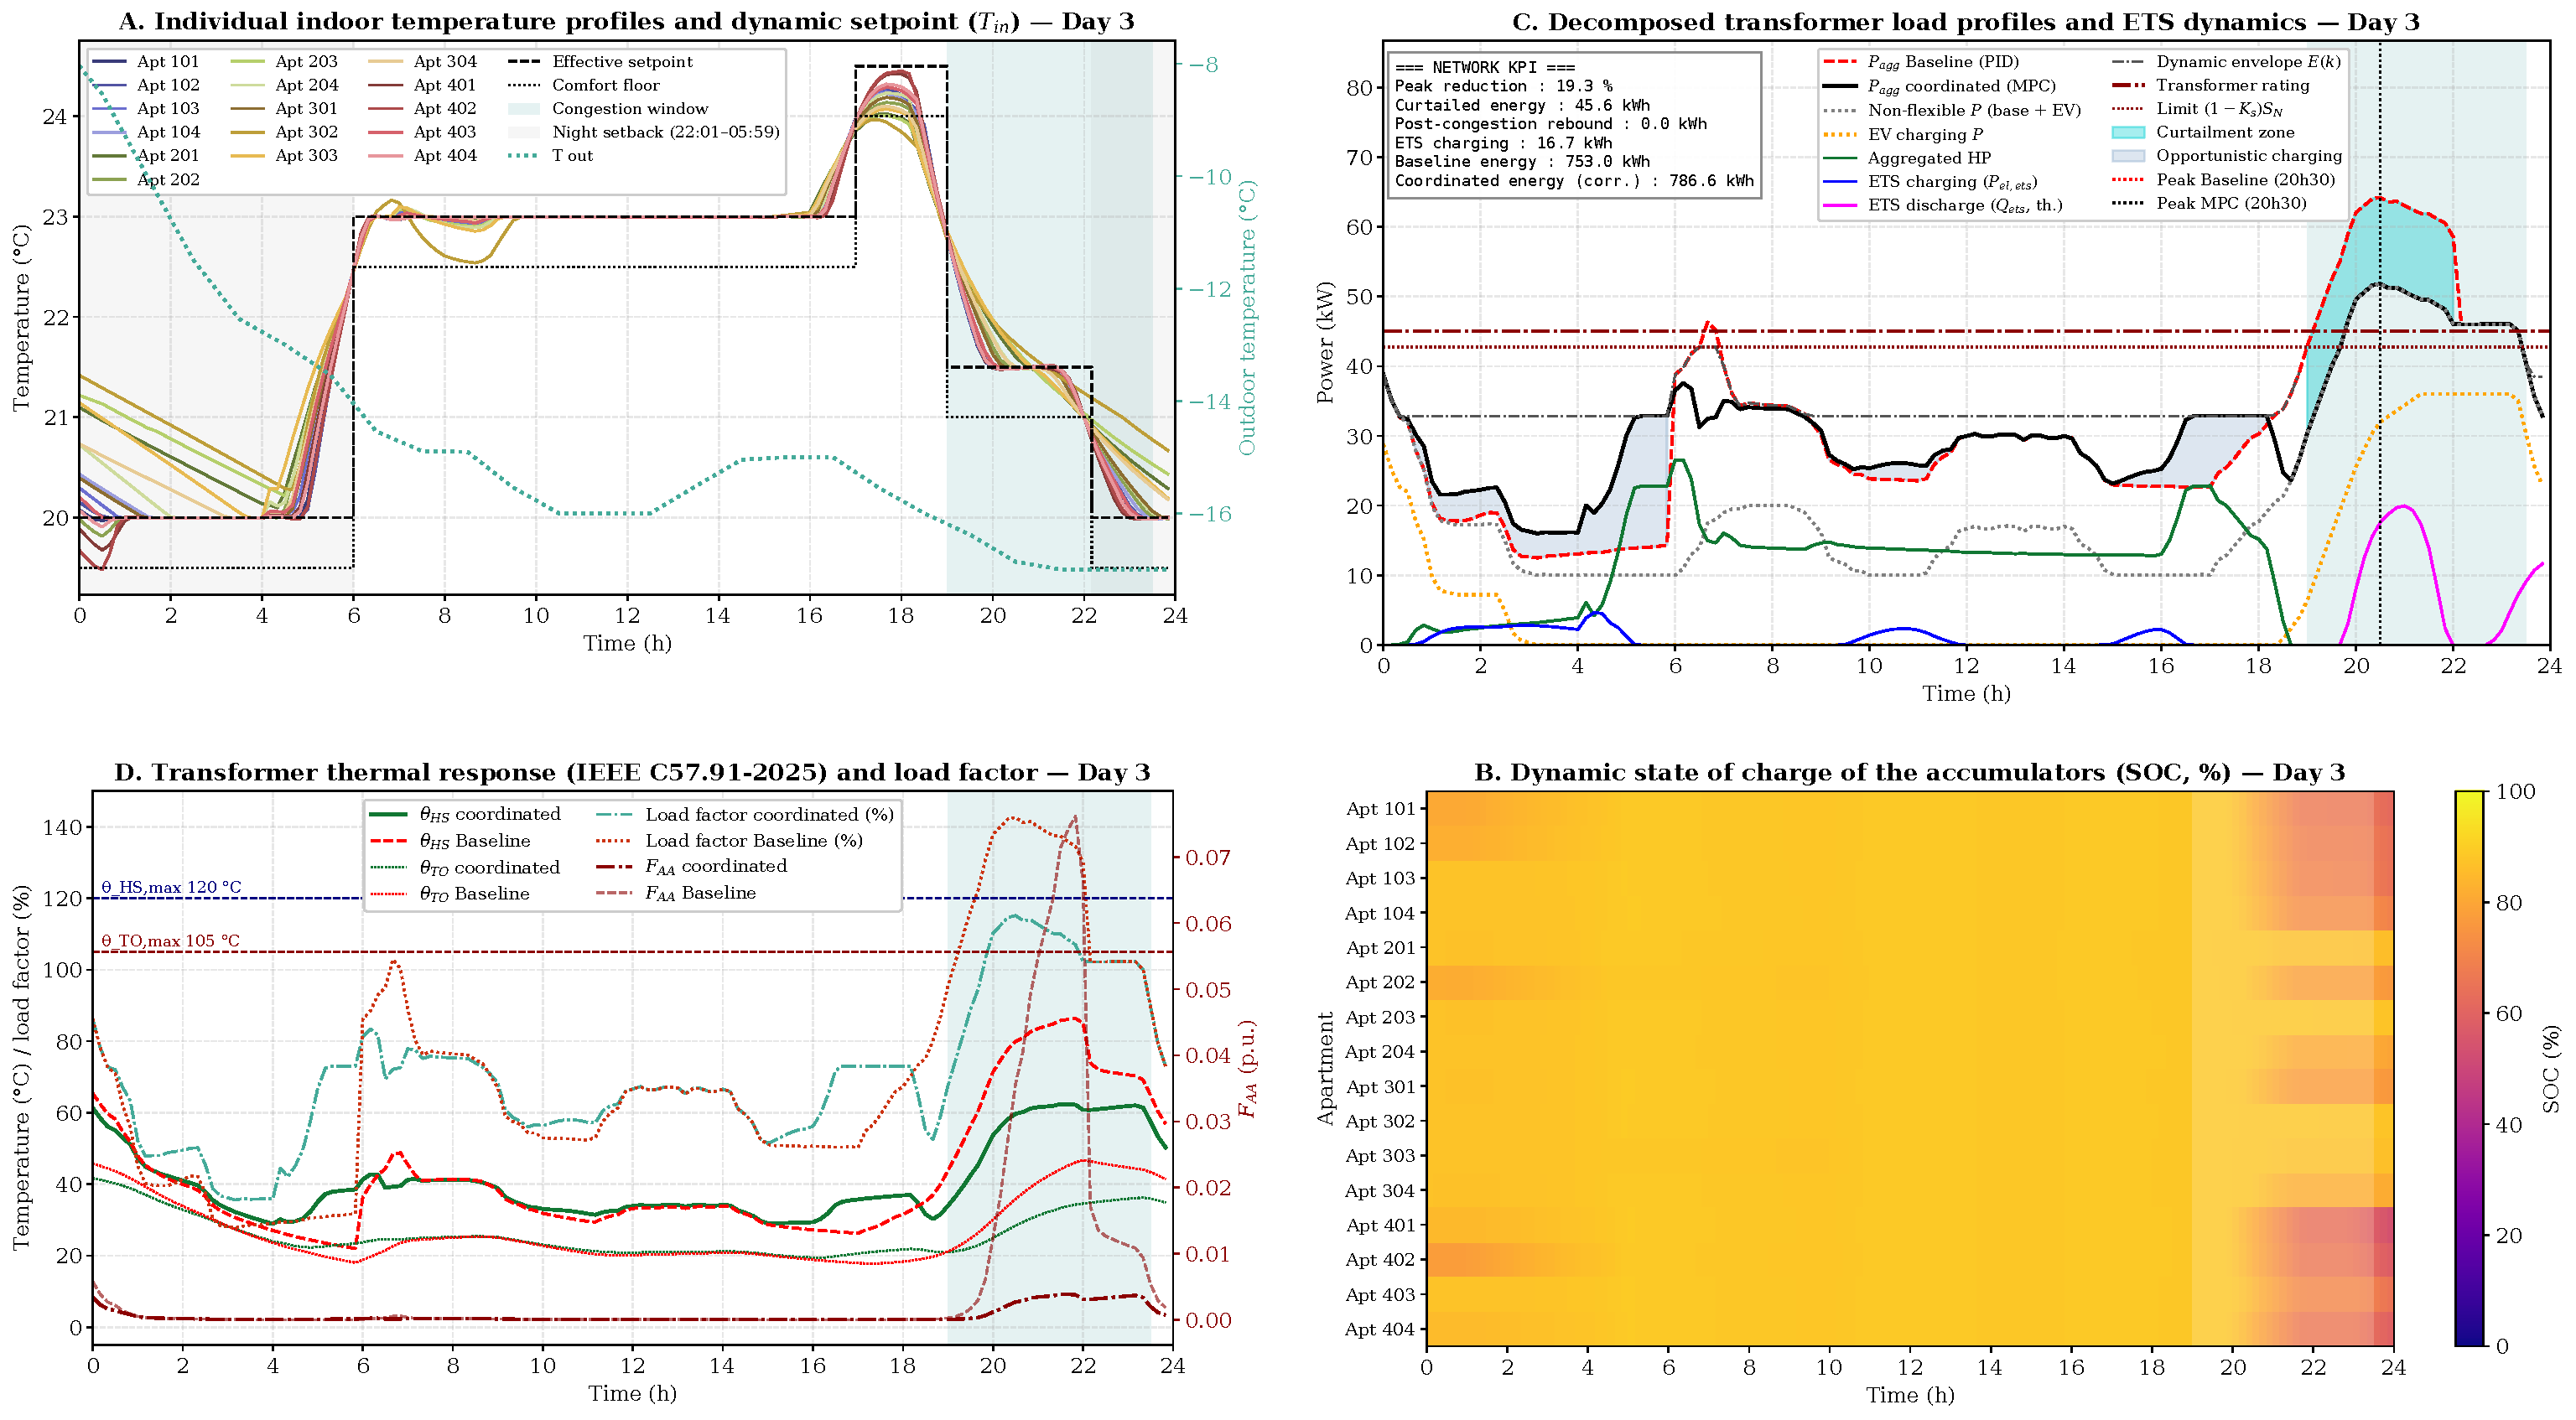
\includegraphics[width=\textwidth,]{fig6_J3.pdf}
\caption{Coordination mechanisms on day 3 (cold snap, −17 to −8 °C). (C) Transformer load decomposition: S0, S1, envelope \(E(k)\), curtailment zone (cyan), opportunistic charging, ETS discharge and aggregated HPs. (D) Transformer thermal response (IEEE C57.91-2025): \(\theta_{TO}\), \(\theta_{HS}\), load factor and \(F_{AA}\) for S0 and S1. Green bands: congestion window.}
\label{fig:6}
\end{figure*}

\subsection{Opportunistic Recharging and Strict Variant}

Off-peak, the coordinated load fills the valleys of the reference---mainly during the night setback, when reference HPs are almost idle---without ever exceeding the envelope: \(\max(P_{coord}-E)=0.00\) kW on all three days, which numerically confirms Proposition 1. Locally, \(P_{coord}\) may exceed \(P_B\) by 12.6 to 18.9 kW, but only within these valleys, and the off-peak maximum actually \textbf{decreases} (41.8 → 40.3 kW on day 3) because the MPC anticipates the 06:00 reheat that the PID concentrates into a step. No rebound is observed, and 74--88 \% of ETS recharging occurs off-peak (Table~\ref{tab:V}). The strict variant confirms the Remark of Section III-D: without valley filling, the off-peak margin is nearly zero, the ETS units receive only 1.0--3.8 kWh\(_e\) per day and become depleted (minimum SOC of 39 \%, 17 \% and then 0 \%). The peak is the same as in S1, but discomfort reaches 80.5, 100.8 and 169.1 °C·h, i.e., 29 to more than 1,500 times that of S1: bounded valley filling is the condition for the strategy to be sustainable.

\subsection{Transformer Thermal Signal}

Coordination lowers the maximum \(\theta_{HS}\) by 16.4--24.0 K depending on the day (Table~\ref{tab:V}, Fig.~\ref{fig:5}-D). In winter, however, \(\theta_{HS}\) stays far below 120 °C even in S0, the cold ambient cooling the unit (its maximum, 101.5 °C, occurs on the \textbf{mildest} day), and the loss of life stays below \(5\times10^{-4}\) \%/day versus 0.013 \%/day for normal aging. The aging term of \eqref{eq:9} is thus inactive and the binding constraint is the \textbf{current}, which motivates a dynamic-thermal-rating envelope allowing temporary overloads in cold weather.

\subsection{Fairness and Robustness}

Ground-floor (slab-on-grade) and top-floor (roof) dwellings, which have the largest conductance \(G_n\), contribute more (6.8--7.4 \% each on day 3) than those on intermediate floors (4.6--5.9 \%). The FCI closely follows the share \(\gamma_n\): Jain's index is 0.980, 0.991 and 0.997 depending on the day.

Finally, with the identified set of Table~\ref{tab:II} and a retuned PI reference, the coordinated peak is identical (set by \(P_{nf}\)) and the reduction still equals the heating share of the reference peak (10--16 \% vs.~15--19 \%); the lighter envelope relies more on the ETS (34--88 vs.~5--37 kWh\(_{th}\)/day, minimum SOC 37 \% at −17 °C). The conclusions are thus robust to the parameter set.

\section{\textbf{Conclusion}}

This paper proposed a hierarchical predictive coordination that successively mobilizes the envelope of a multi-unit residential building, preheated by HPs, and refractory-brick electric thermal storage units to relieve a 50 kVA distribution transformer during winter peaks. Three results emerge from the 72 h simulation of a 16-unit MUB. First, the peak is reduced by 14.8--19.3 \%, exactly the heating share of the reference peak: when EV charging alone exceeds the transformer capacity, thermal flexibility reaches a physical ceiling. Second, the maximum hot-spot temperature drops by 16--24 K, but remains far below 120 °C in winter, so the active constraint is the current rather than aging. Third, these gains are obtained without artificial peak or rebound, with improved comfort (82--99 \% less discomfort), high fairness (Jain's index ≥ 0.98) and a 1.4--4.5 \% energy penalty due to the HP → ETS substitution. For a distribution utility, ETS recharging can thus be confined under the reference without creating an artificial peak, provided bounded valley filling is allowed; the strict variant, which forbids it, depletes the storage units.

These results rely on perfect forecasts, a preliminary parameter set and deterministic EV profiles. Future work will address a dynamic power envelope derived from the transformer thermal model, joint coordination of EV charging, stochastic control under forecast errors \cite{Oldewurtel2012}, a comparison of identification methods under parameter degradation, and hardware-in-the-loop validation.

\section*{\textbf{Acknowledgment}}
The authors would like to express their sincere gratitude to their industrial partners, particularly \textbf{Hydro-Québec}, for its support and for providing the favorable conditions that made this research possible. They also wish to thank the administration of the \textbf{Université du Québec à Trois-Rivières (UQTR)}, as well as the entire team of the \textbf{Laboratory for Innovation and Research in Intelligent Energy (LIREI)}. Special thanks are extended to \textbf{Rasmané Bandé} for his valuable collaboration, availability, and generous sharing of knowledge and information.
\addcontentsline{toc}{section}{Acknowledgment}

\bibliographystyle{IEEEtran}
\bibliography{refs}
\end{document}
